\chapter{Statusseminar}



\section{Indledning}
% baggrund for projektet
Artrose er den mest udbredte gigtsygdom og en af de mest udbredte kroniske sygdomme i Danmark 
%(\textbf{Note: tilføj hvad en kronisk sygdom er}) \citep{sygdom}. 
Artrose er en kronisk ledsygdom der kan ramme alle ledstrukturer, men primært rammes ledfladernes bruskdele \citep{schroder}. Prævalensen for artrose i Danmark er omkring 800.000 personer, og der sker årligt over 20.000 indlæggelser med artrose aktionsdiagnose. \citep{sygdom}
Forekomsten af artrose stiger med alderen, hvor personer over 55 år repræsentere den største gruppe af artrose patienter. Over de seneste 15 år er der sket en stigning i artrose operationer fra 2500 i år 2000, til over 9000 i år 2015. \citep{aarsrapport2016} \\
Af artrose lidelser er knæartose en af de hyppigst forekommende. Denne form for artrose er den førende årsag til funktionsnedsættelse i de nedre ekstremiteter \cite{bezwick2012}. 
Knæartrose medfører at ledbrusken nedbrydes, samtidig med at der forløber en række reaktioner i knoglen under brusken, samt i synovialmembranen \citep{brostrom2012}. Som følge af den tiltagende bruskmangel kan der opstå ledskurren og fejlsstilling, hvilket kan medføre belastningssmerter og i sidste ende funktionstab \citep{ugeskrift2011}.
Der er stor variation i hvordan personer der lever med knæartrose påvirkes, og nogle vil derfor kunne leve relativt upåvirkede med sygdommen, mens andre vil opleve at sygdommen svækker både arbejdsevne og livskvalitet \citep{sygdom}.
Generalt for knæartrose oplever patienter smerter i knæleddet. Smerterne varierer meget, og kan gå fra at være let irritable til uudholdelige. Knæartose patienter kommer igennem et længere bahandlingsforløb, men da knæartrose er irreversibel, kan artrose kun afhjælpes og ikke kurreres, og de fleste ender med at få en total knæalloplastik (TKA). 
% intro til projektet
Ifølge sundhedsstyrelsens vurdering er knæalloplastik, effektiv til at mindske smerte, øge funktion og derved bedre livskvalitet, og idet TKA-operationen er den sidste behandlingsmulighed, er operationstilfredshed en betydningsfuld problematik. %det vigtigt at opnå dette mål. Det ses dog hos TKA-patienter at 19\% efter den primære operation og 47\% efter revision fortsat oplever svære smerter \citep{Petersen2015}. 
Et studie af \cite{Bourne2010} viser imidlertid, at 11 til 25\% af TKA-patienter generelt er utilfredse efter operationen, hvorved behandlingen fra et patientøjemed ikke vurderes som succesfuldt.
Modsat ses det af sundhedsstyrelsens årsrapport for totale knæalloplastikoperationer at alle succeskriterier overholdes for alle operationer. \citep{aarsrapport2016} 
Der opstår således et dilemma i at behandlingen af knæartrose, set fra sygehusvæsenets perspektiv, er succesfuldt, men fra patientens synspunkt er mislykket.
Der opstilles derfor en initierende problemstilling:

\subsection*{Initierende problemstilling}
\begin{center}
	\textit{Hvorfor oplever 11 til 25\% af TKA-patienter kroniske postoperative smerter?}
\end{center}


\section{Problemanalyse}

\subsection{Patientmålgruppe}

En længere række faktorer har betydning for udviklingen af artrose. Hvis en eller flere af disse faktorer er tilstede, er den påvirkede mere disponeret for knæartrose. Dette er eksempelvis, overbelastning igennem arbejde og fritid, tidligere knæskader, genetisk arv, overvægt samt køn \citep{brostrom2012}. Knæartrose er til stede blandt 45\% af alle 80-årige i befolkningen. Antallet af personer med knæartose kan formodes at stige da levealderen i Danmark stiger. Dette er ikke det eneste faktor, hvorfor prævalensen kan antages at stige. En af risikofaktorerne for udviklingen af knæartrose er overvægt, hvilket 47\% af den danske befolkning kan kategoriseres som. Ydermere stiger andelen af overvægtige med alderen, hvilket ligeledes er tilfældet for knæartrose. Overvægtige med en høj body-mass-index (BMI>30\citep{definitionfedme1999}) er disponeret for knæartrose med en relativ risiko på en faktor tre, hvoraf en kombination af ovenstående faktorer øger risikoen for lidelsen. Dog kan der opstå problematikker vedrørende benyttelsen af BMI, da metoden ikke skelner mellem fedt og muskler. \textbf{(8)} \citep{brostrom2012} \citep{Vestergaard2014} \citep{Vestergaard2016} \citep{Lind2016} \citep{Lind2016b}

En patients symptomer kan medføre igangsættelsen af et behandlingsforløb. Et behandlingsforløb for en patient med knæartrose består af flere faser, hvis mål er smertelindring, mobilitetsforøgelse samt forebyggelse. Generelt kan faserne opdeles i non-invasive og invasive metoder. Hvilken metode som hjælper patienten afhænger af graden af knæartrose.

\begin{figure}[H]
	\centering
	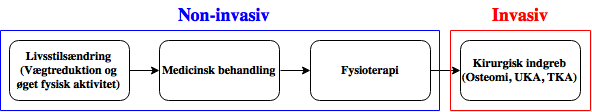
\includegraphics[width=1\textwidth]{figures/bProblemanalyse/flowchart_behandlingsforloeb.png}
	\caption{På figuren ses et flowchart indeholdende de forskellige behandlingsmetoder der forekommer igennem et patientforløb med knæartrose.}
	\label{fig:flow_behandlingsfaser}
\end{figure}\vspace{-.25cm}

Patientgruppen som postoperativt er utilfredse er svært definerbar. Problematikken opstår i og med klassificeringen bag de potentielt 11 til 25~\% utilfredse patienter er vedrørende postoperative smerte samt funktion. Det kan forestilles at der blandt nogle af patienterne findes en forventningsfaktor, hvilket gør de postoperativt kategoriserer sig selv som værende utilfreds, omend de rent faktisk har opnået en forbedring af både smerte og eller mobilitet. Det kan tænkes at forventningsfaktoren kan være medvirkende til at kategorisere dem som værende utilfredse, som resultat af skuffelsen af ikke at fungere som et individ med et fuldt funktionsdygtigt knæ. Denne antagelse understøttes af \cite{Bourne2010}, som beskriver de største prædiktorer omhandlende utilfredshed efterfulgt af en TKA-operation. Den faktor som besidder den største score er, patientens forventninger til operationen ikke er mødt, hvilket medfører 10,7 gange større risiko for utilfredshed. \citep{Bourne2010} I et andet studie af \cite{Keudell2013} bliver patienternes alder sammenkoblet med deres forventninger. Det tyder på at den ældre patientgruppe (>65 år) har generelt har lavere forventninger til operationsresultatet, end den yngre patientgruppe (<55 år). I dette studie indikeres det at den ældre patientgruppe generelt har større tilfredshed, end den yngre. Dette kan antages at have en sammenhæng med påstanden fra \cite{Bourne2010}, vedrørende prædiktoren til utilfredshed, omhandlende forventninger til operationen. \textbf{NOTE:(7 (mangler analyse?))}

\subsection{Non-kirurgisk og kirurgisk behandling}

Artrose kan som tidligere nævnt ikke helbredes, og non-kirurgiske behandlingsmetoder vil derfor fortrinsvis søge at smertelindre samt forbedre funktionen af knæet \citep{brostrom2012}. En essentiel del af behandling af knæartrose, består af at informere og uddanne patienten, med henblik på at patienten opnår indsigt i sygdommen, samt at patienten aktiv inddrages i behandlingsforløbet. I behandlingsforløbet er træning ligeledes en vigtig faktor, både før og efter en eventuel operationen. Dette afspejles i både nationale og internationale kliniske retningslinjer, hvor der er bred konsensus om, at træning er af væsentlig betydning ved behandling af knæartrose \citep{brostrom2012}. Smertestillende medicin er ligeledes en stor del af behandlingen, da patienter ofte ikke har mulighed for at træne, på grund af alder, vægt, aktivitetsniveau.\\

Kirurgiske behandlingsmetoder indebære osteotomi og knæalloplastik. Osteotomi har tilformål at afhjælpe den mekaniske belastning i det berørte område, for derved at afhjælpe smerterne. Ved osteotomi fjernes der oftest en kile af tibia-knoglen og det resterende knogle sikres med skruer og metal plader. Proceduren ændre knæets mekaniske akse, hvilket vil ændre belastningen af de degenererede områder. \citep{Osteotomi_og_TKA}
Alloplastik er et operativt indgreb der har til formål helt eller delvist at udskifte knæleddet, med specielt designede metal- og plastkomponenter som varig erstatning for bruskfladerne i knæet. Operationen opdeles i TKA og UKA, hvilket henholdsvis er helt eller delvis udskiftning af knæleddet og afhænger af den specifikke diagnose. Der kan ved traume tilfælde eller svære beskadigelser af de anatomiske strukturer omkring knæet forekomme specialiserede udgaver af knæalloplastik.

\begin{figure}[H] 
	\begin{center}
		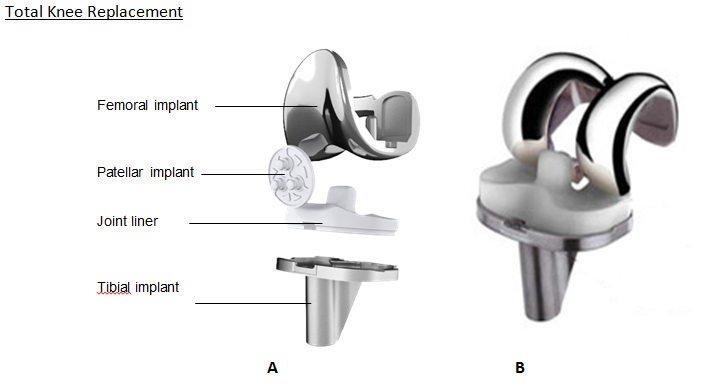
\includegraphics[width=0.7\textwidth]{figures/tka_implant}
	\end{center}
	\caption{Komponenterne til en total knæalloplastik, består af et femural og tibia implantat ofte bestående af en titaniumlegering. Patella- og tibiaindsatsen er lavet af polyethylen, hvilket er med til at mindske friktionen og efterligne knæledes naturlige bevægelse.\cite{1}} 
	\label{fig:tka_implant} 
\end{figure}

Efter en vellykket operation burde patienter ikke oplever smerter, dette er imidlertid ikke tilfældet. Der er således et problem med resultatet af operationen, på trods af operationen overholder sundhedsstyrelsens succeskriterier \citep{aarsrapport2016}. Det må derfor antages problemet ikke ligger ved operationen, men da en del patienter oplever postoperative smerter, er det relevant at undersøge smertes indflydelse på resultatet af operationen. 

\subsection{Smerte}





















